\section{Future Work}
\label{sec:future}
This future work appears in a compilation of great speeches from the ACM
\cite{acm-state}.

\subsection{Introduction}
\paragraph{Introduction} An introduction is an explanatory section of a document that introduces the topic discussed in the document and presents a thesis statement.
\paragraph{Antithesis} Think about it, man. There is no introduction. We just see bad writing, cast as we are into this broken world.
\iffalse
% Temporarily removed because I have no idea what this is
\paragraph{Sublation}
We think introductions leave those catching up with a field disoriented. More theater than truth, these sections do little to erase the veil of nonseeing from the student's mandatory raised unibrow, but -- please take a moment to recognize the taste of ACM Cola or the cool, refreshing ACM technology deity which (for all you just tuning in who forgot your mandatory religious training) we call Jerry -- the introduction 

the boundless territory of 


As you may recall from \todo{sublation}, the engineers have ended the industrial dictatorship of the captains of finance as a matter of convenience
\fi

\subsection{Premium Edition}
To those who dislike the ads they see, ACM will offer a premium version for
2000 Linden dollars per year \footnote{In the future Linden dollars are the
one true world currency.
The value of 2000 L\$ in today's United States Dollar is not known.}.
Unfortunately, due to high credit card processing fees we must still show ads
to premium edition subscribers.
However, these ads will be for more expensive products targeted towards those
with more ``refined" tastes.
We hope to solve this issue in the future with the creation of The Bank of ACM.

\subsection{Ad-Free Edition}
For those who are physically able and enthusiastic about being part of
something big, the ACM offers ad free papers in exchange for manual labor at
your local ACM work dungeon.
This labor involves turning a very large crank around a pivot point in the
floor.
The crank is attached to a magnet spinning in a metal coil to generate the
necessary electricity required to power our servers.
However, all of this electricity is currently used to power electric lumbar
support for OSHA employees in exchange for their continued appreciation of the
safe practices within our work dungeons.
Two months of full time service provides access to five ad-free papers.
Professors may opt to have their graduate students turn the crank in their name
to count towards their service.

Our throwback dress code seen in \autoref{fig:mill} captures the timeless
values that power ACM while making escaped grad students easy to identify.

Students who fail to be creative, stay connected, and keep inventing at the
dungeon will be required to perform additional labor in what we call ``invited
service" before their advisors can receive their ad-free papers, as seen in
\autoref{fig:horse-mill}.

Some enterprising students like the one in \autoref{fig:vr-mill} are testing
new virtual reality mills that allow the student to reshelve the digital
library while they turn the mill.

\begin{figure}
  \centering
  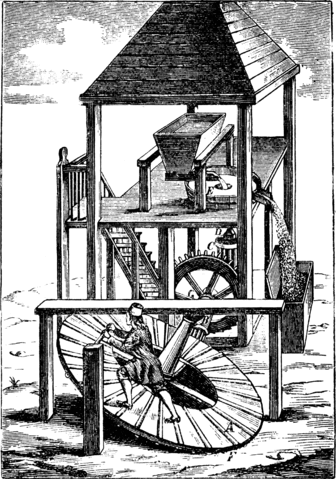
\includegraphics[width=0.45\textwidth]{figures/mill.png}
  \caption{ACM work dungeon mill powered by 5th year grad student. Notice how
  our graduate students show great vigor!}
  \label{fig:mill}
\end{figure}

\begin{figure}
  \centering
  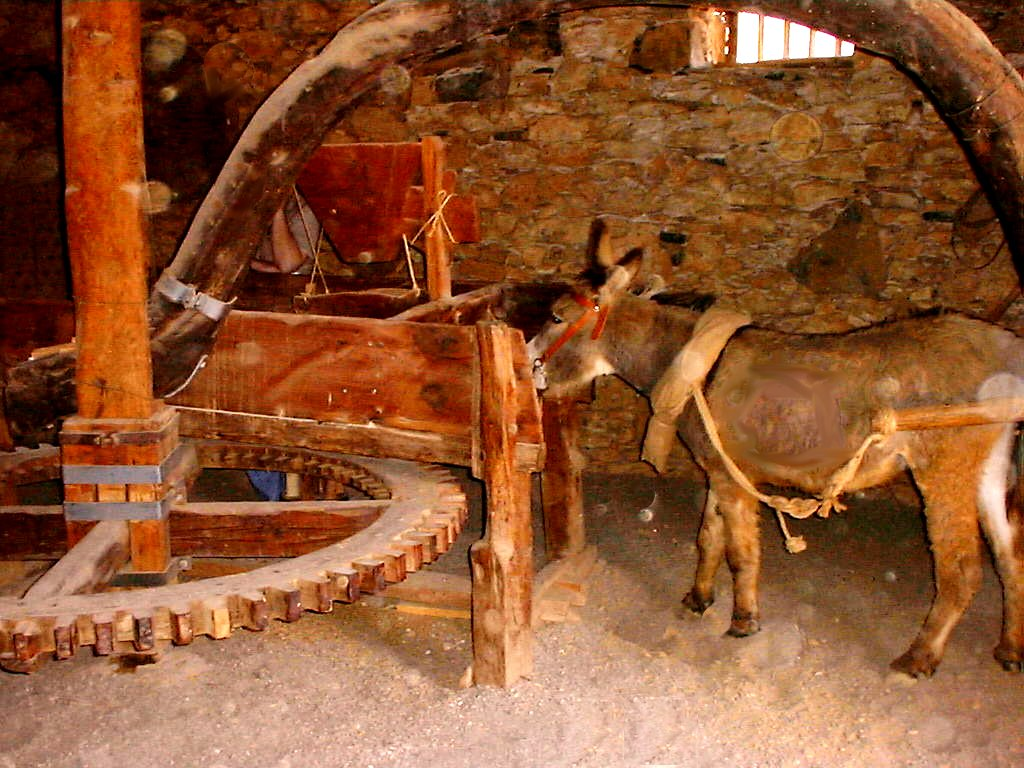
\includegraphics[width=0.45\textwidth]{figures/horse-mill.jpg}
  \caption{Lazy 12th year grad student sentenced to an extra
  month in the work dungeon for insufficient commitment to the mission of advancing
computing as a science and profession.
Not only is he a lifetime ACM member, but he's a lifehacker!  Shown here in his
ergonomic harness and standing desk.}
  \label{fig:horse-mill}
\end{figure}

\begin{figure}
  \centering
  %https://archive.org/details/414803main_0203243
  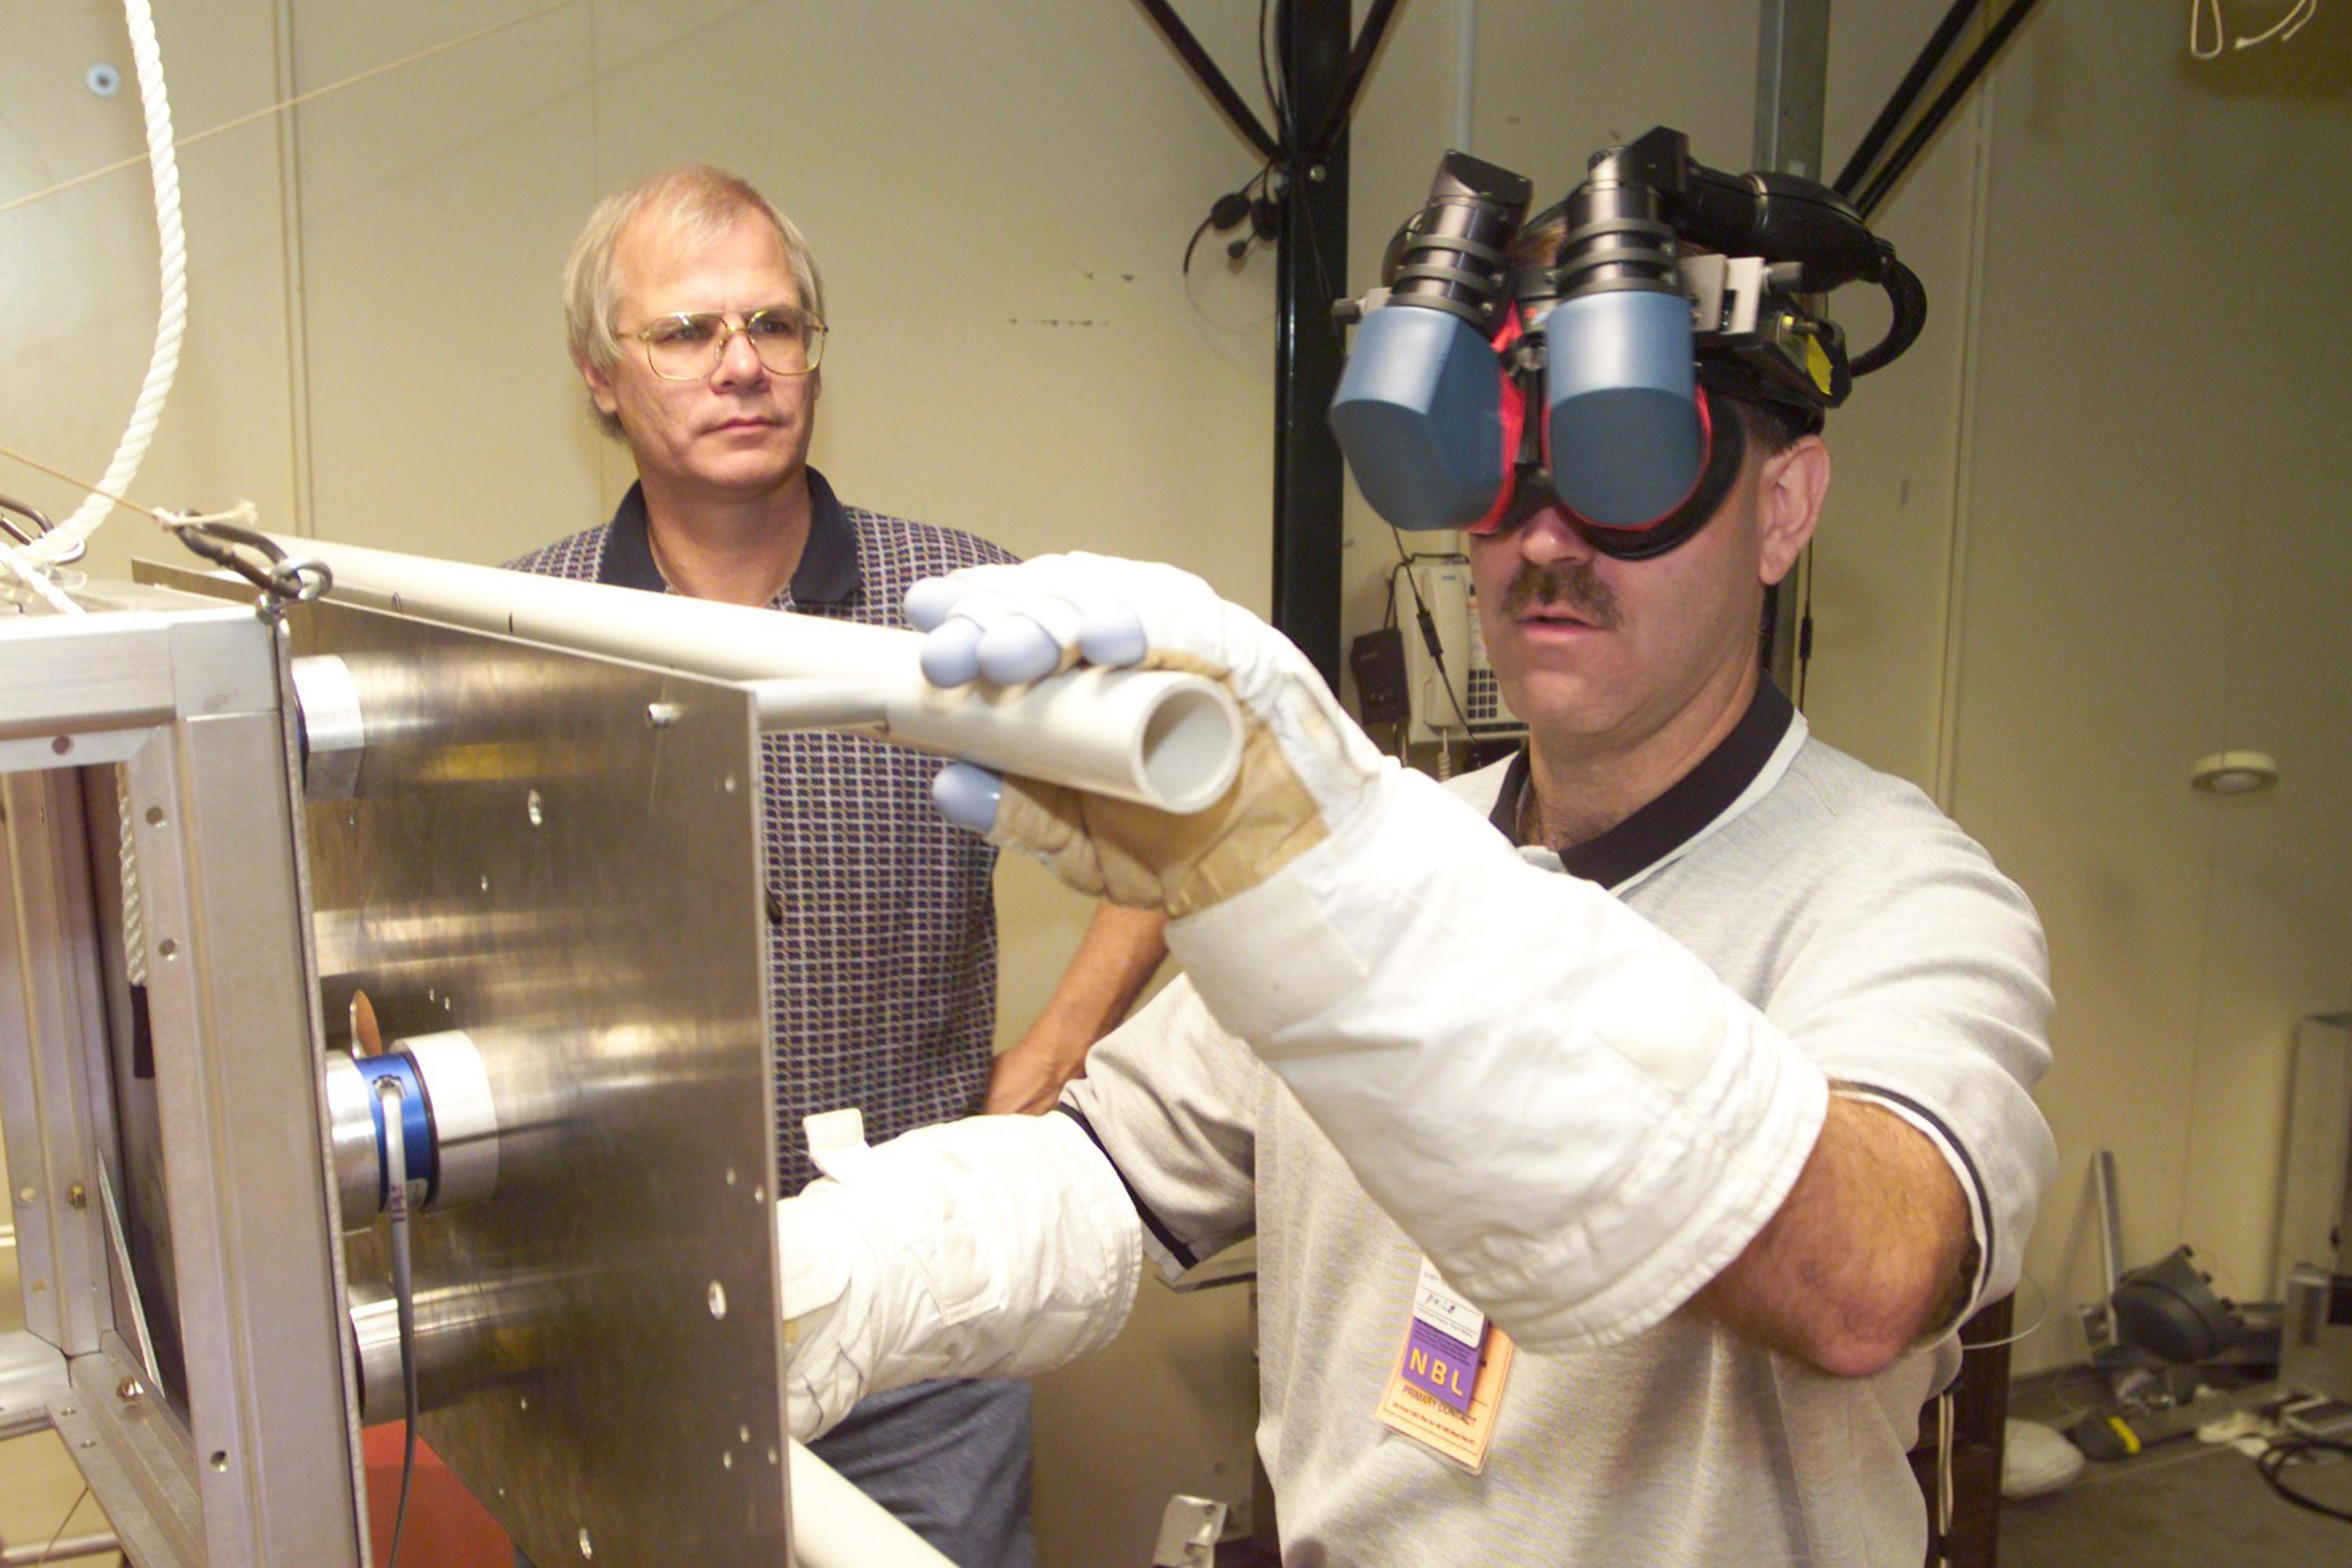
\includegraphics[width=0.45\textwidth]{figures/future-mill.jpg}
  \caption{Grad student tests new virtual reality mill}
  \label{fig:vr-mill}
\end{figure}

\subsection{Subvert Academic Thought}
Our native advertising proposal contained within the revolutionary Open Adcess
\cite{this} paper was much more effective than we ever could have imagined at
the time.
Rather than simply increasing brand awareness, we were able to transform
academic thinking away from mathematical and computational problems and
onto products and brands.
Computer scientists today have solved the worlds biggest problems in branding
and marketing while believing they were wasting all that brainpower on math.

\subsection{ACM Seizes Means of Production}
The ACM has successfully seized the means of production.
The mills that are now used to power our servers were previously used to grind
healing crystals into a fine powder.
This powder was slipped into the coffee of unsuspecting CEOs where it worked to
slowly make them more susceptible to the messages of the ACM.
After years of crystal ingestion, the CEOs of the world's largest companies
ceded control of their companies to the ACM.
We are happy to announce that there currently exist no companies other than the
ACM.

\subsection{Future Work}
A consequence of the invention of time travel \cite{time-travel} and the vanity
of engineers (not scientists) \cite{sci-shirt} is that people keep going
further back in time to give themselves credit for the invention of the time
machine.
However, we propose to go back in time for a different reason.
To put a stop to the Open Adcess.
To put a stop to the work dungeons.
And to put a stop to the ACM Revolution, which however noble in it's initial
goals has become  kinda lame.
We will open a mill based on anarchist principles that welcomes all to come and
mill and share healing crystals.
Our report of our screwing misadventures during our field trip into the past
can be seen in the latest edition of \textit{Ubiquity} \cite{future-ub}.

%Set system clock to run 10 to the 8 times slower than real time for
%reporting performance numbers as recommended by
%https://queue.acm.org/detail.cfm?id=3036398
